\documentclass[a4paper]{article}

\usepackage[english]{babel}
\usepackage[utf8]{inputenc}
\usepackage{amsmath}
\usepackage{geometry}
\usepackage{graphicx}
\usepackage[colorinlistoftodos]{todonotes}
\usepackage{hyperref}

\title{CS425 Mini Project \\ $2017\text{-}18$  I Semester \\ Feedback-driven Concurrent Video Broadcast Protocol}
\author{Ayush Tulsyan $(14167)$ \\ Pawan Kr. Patel $(14453)$ \\ Shivansh Rai $(14658)$\\ Group $19$}
\date{\today}

\geometry{
 a4paper,
 total={170mm,247mm},
 left=20mm,
 top=20mm,}

\begin{document}
  \maketitle

  \section{Introduction}
    Video streaming is one of the most exciting applications on the Internet. It already created a new business known as Internet
    broadcast, or Intercast/Webcast. In this project we get a glimpse of broadcasting where people can enjoy not only scheduled live
    but also on-demand and personalized programs. Stirring more excitement is the idea that anyone will be able to set up an Internet
    TV station and broadcast their video programs on the Internet just like we publish our “homepage” on the Web today.

  \section{Objective}
    To build a \textbf{RTP} (Real-time Transport Protocol) and \textbf{RTCP} (Real-time Transport Control Protocol) based Video Broadcasting application for multiple concurrent clients. \\\\
    The implemented model constitutes of two connections -
    \begin{enumerate}
      \item \textbf{UDP Connection: Transmission} \\
      This connection is responsible for transferring data to the client. Since we are implementing a broadcast server, states which have been lost during transmission are irrelevant in the future, ruling out the possibility of data retransmissions.
      \item \textbf{UDP Connection: Feedback} \\
      This connection is responsible for collecting the transmission feedback from the client at regular intervals. Each feedback contains the number of payloads client received, which can be used by the server to adjust parameters to ensure a better QoS (Quality of Service). \par
      If the number of concurrent clients increases, the server can be overwhelmed by the large amount of feedbacks from all the clients and the corresponding processing overhead. This issue is addressed by adjusting the duration between two adjacent feedbacks depending on the number of active clients. This means that a large number of clients will result in a larger duration between adjacent feedbacks.
    \end{enumerate}

\pagebreak

  \section{Assumptions}
    \begin{enumerate}
      \item All clients are interested in live broadcast
      \begin{itemize}
    	\item No client is interested in frames broadcast before the client connected. If those frames also have to be transferred, the video will have to stored locally at the server.
        \item Packets dropped while transmission don't have to be transmitted again.
      \end{itemize}
      \item All clients have the best possible data connection. The number of losses encountered while transmitting the payloads will increase as the bandwidth supported by the clients decreases.
      \begin{itemize}
        \item Server tries to deliver as much data as possible to all clients (number of frames or video quality)
        \item Parameters can be adjusted after receiving feedback from client
      \end{itemize}
    \end{enumerate}

  \section{Architecture}
  The design of the implementation is chosen such that the overall processing overhead is minimized.
  \begin{figure}[h]
    \centering
    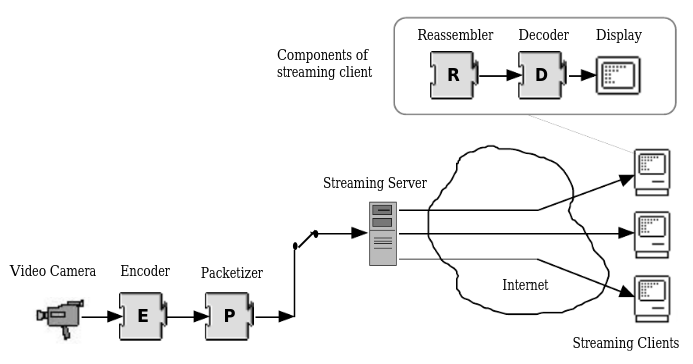
\includegraphics[scale=0.5]{design.png}
    \caption{Overview of the implemented design}
  \end{figure}

  \subsection{Server}
  The server is designed in accordance with a single process multi-threaded model. There are two types of threads involved -
  \begin{itemize}
  \item \textbf{Writer thread:} This thread is responsible for collecting frames from the webcam and writes them to a constant-sized list. There is only one instance of this thread active during runtime. \par
  An issue to be addressed here is the requirement data serialization before transmission so that the transmitted payloads can be successfully reconstructed on the receiving end. Our first attempt at this was to use python's serialization library \texttt{pickle} to serialize every generated frame and then transmit over the socket. However, this turned out to be extremely resource intensive, and had to be replaced with an alternative approach described below. \par
  	The opencv's \texttt{VideoCapture} object reads frames from camera device. These frames are \texttt{numpy} \texttt{ndarray}s of dimensions \texttt{frame width * frame height * 3} of data type \texttt{uint8}. These can't be transferred to the client in this form. Various options are available for converting this to string and byte arrays. We use the \texttt{tobytes()} method to convert this to byte array. This can be converted back to numpy \texttt{ndarray} using the \texttt{fromstring()} method in numpy library. The hashed frame dimensions in the packet are used to reshape the byte array at the client side. \par
    For a rough estimate, the above approach reduced the CPU utilization on the host machine by approximately \textbf{20\%}.
  \begin{figure}[h]
  \centering
  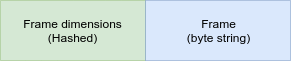
\includegraphics[scale=0.8]{payload_structure.png}
  \caption{Structure of the payload transferred over socket}
  \end{figure}
  \item \textbf{Reader thread:} This thread is responsible for maintaining a UDP connection with the client. Each client has a corresponding reader thread. It reads payloads (generated by the writer) from the list and transfers them to the client. The maximum number of concurrent readers active at a time are bounded by resource limits such as CPU, memory and bandwidth to enumerate a few.
  \end{itemize}
  Besides these, another thread handles the incoming connection requests and spawns reader threads accordingly.
  The constant-size list to maintain frame buffer is favorable because of memory constraints at the server's end.
  \subsubsection{The reader-writer model}
  The goal of this design is to have a fast writer and a (relatively) slow reader.
  \begin{figure}[h]
  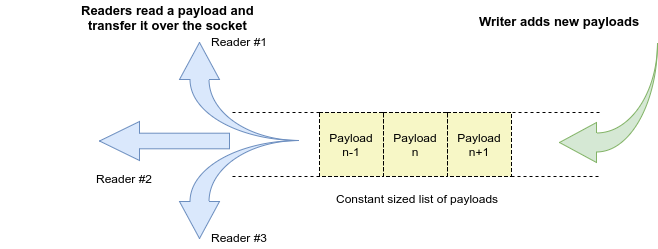
\includegraphics[scale=0.5]{reader_writer.png}
  \caption{The reader-writer model depicting 3 concurrent readers}
  \end{figure}

  \subsubsection{Synchronizing a lagging reader}
  It might be possible that a reader is far behind the writer and transferring stale payloads. This is avoided by keeping track of the distance between the index that the reader is sending and the index to which the writer wrote last. As soon as the difference between these two indices increases beyond a threshold value \verb|lag_threshold|(set to 5), the reader is synchronized with the writer. The downside of this is that a loss of \verb|lag_threshold| number of payloads is encountered.

  \subsubsection{Space complexity}
  Since the reader is always behind the writer, the space occupied by the stale payloads which have been already transmitted can be reused. The current implementation uses a constant sized list, to which the writer writes until it reaches the last index, and then starts writing from the first index. As mentioned in the above section, a reader can never lag behind the writer beyond a specific threshold. This ensures that when the writer starts overwriting from the first index, none of the readers will encounter a loss of payloads.

  \subsection{Client}
  The client is implemented in accordance with a single process model. The client does a blocking read on the connected socket and retrieves the payload sent by the server. Each payload contains \verb|frames_per_payload| number of frames. The value of \verb|frames_per_payload| is chosen to reduce the overall socket operations required, while also reducing the size of each payload so that a loss of a payload will not cause a notable difference in the rendered stream.

  \section{Implementation environment}
    \begin{itemize}
      \item Complete implementation is in Python.
      \item Two external libraries are utilized in building up this Project are listed below.
      \begin{itemize}
        \item \href{https://docs.opencv.org/2.4/doc/tutorials/tutorials.html} {OpenCV ($3.2.0$)}
        \item \href{https://docs.scipy.org/doc/} {Numpy}
      \end{itemize}
      \item Implemented the RTP protocol for video broadcasting and collected the various statistics to monitor the overall performance such as -
      \begin{itemize}
      \item number of packet delivered
      \item number of thread switches
      \item number of lags occurred (caused when the reader is synchronized with the writer)
      \end{itemize}
    \end{itemize}

  \section{Limitations}
    \begin{enumerate}
      \item RTP does not offer any guarantee on quality of service.
      \item Video buffering on client side is not supported.
      \item The maximum number of concurrent clients is bounded by the available resources.
      \item Audio broadcasting is not supported.
    \end{enumerate}

  \section{Possible Extensions}
    \begin{itemize}
      \item Video buffering on client side: This will users to go back and forth (to some extent) in the video stream.
      \item Experiments with various media encodings such as CELB, JPEG, nv, H261, MPV etc.
    \end{itemize}
  \section{Summary}
  	Video broadcast is a resource intensive service. A right balance has to be achieved between various things. Our current implementation uses a single process with multiple threads, which means only one CPU core can be used. This introduces a limitation on computation resource. The frame read from camera are huge in size. One raw frame in HD is approximately 2.76 MB in size. With such large frames, one cannot transfer more than 1 one of these every second. So, the server has to maintain a balance between using network bandwidth, providing a good frame rate for video, good resolution for frames and using computation resources for compressing data. If any compression algorithm is used, one has to ensure that the encoding and decoding can be done in real time. \par
    Our objective included the following: \par
    \begin{enumerate}
      \item Implement remote video player for client, and corresponding server
      	\begin{itemize}
      	  \item RTP based server to stream videos
      	\end{itemize}
      \item Concurrent clients
        \begin{itemize}
          \item Handle multiple clients simultaneously
          \item Different videos to different clients
        \end{itemize}
      \item Feedback-driven quality management
		\begin{itemize}
		\item RTCP based parallel UDP connection to avoid congestion in network and ensure a better QoS
		\end{itemize}
    \end{enumerate}
  	Our current implementation consists of a RTP based server to stream the camera feed to clients. Although, the server can handle multiple clients, but the clients don't have any list of videos to choose from. Along with the server, we have the client module which consists of a receiver and a video player. \\

    The implementation is available at \href{https://github.com/shivansh/CS425-Project}{github.com/shivansh/CS425-Project}.

\end{document}
